\title{Programação Para Web: Apresentação da Disciplina}
\date{\today}
\frame{\titlepage}

\begin{frame}[fragile]
  \frametitle{Objetivos Gerais - Prog Web}
  \begin{itemize}
    \item Proporcionar uma compreensão abrangente da arquitetura cliente-servidor e das tecnologias web fundamentais.
    \item Desenvolver habilidades práticas em programação web, utilizando linguagens de marcação, estilização e script.
    \item Introduzir metodologias modernas de desenvolvimento web, incluindo o uso de frameworks como React.js e ferramentas como Git e GitHub.
    \item Fomentar a capacidade de construir e manter aplicações web acessíveis, responsivas e de alta qualidade.
  \end{itemize}
\end{frame}

\begin{frame}[fragile]
  \frametitle{Objetivos Específicos}
  \begin{itemize}
    \item Semana 1-4: Dominar os conceitos básicos da Web, protocolos web, HTML5, CSS e introdução ao JavaScript e TypeScript.
    \item Semana 5-8: Desenvolver aplicações interativas com React.js, compreendendo componentes, estados e props, além da modularização e reutilização de componentes.
    \item Semana 9-12: Aplicar estilos avançados e design responsivo em projetos web, utilizando CSS in JS e bibliotecas como Styled-components. Praticar usabilidade e acessibilidade.
    \item Semana 13-16: Implementar e documentar projetos práticos integrando com APIs RESTful, focando em padrões de interoperabilidade de dados e estilos arquiteturais web.
    \item Semana 17-18: Avaliação prática e teórica para consolidar os conhecimentos adquiridos e introdução a conceitos avançados de arquitetura de software.
  \end{itemize}
\end{frame}

\begin{frame}[fragile]
  \frametitle{Motivação da Disciplina}
  \textbf{Por Que Estudar Programação para Web?}
  \begin{itemize}
    \item Em um mundo cada vez mais digital, o desenvolvimento web se tornou essencial para a criação de soluções inovadoras e eficientes.
    \item Esta disciplina oferece uma \textit{visão panorâmica} das tecnologias e práticas fundamentais no desenvolvimento frontend, preparando os alunos para os desafios reais do mercado.
    \item O conteúdo abrangente, embora introdutório, permite que os alunos \textit{identifiquem suas áreas de interesse} e especialização futura no vasto campo da engenharia de software.
  \end{itemize}
\end{frame}

\begin{frame}[fragile]
  \frametitle{Objetivo da Visão "Rasa" na Aprendizagem}
  \textbf{Entendendo o Básico: Uma Fundação para o Futuro}
  \begin{itemize}
    \item Ao adotar uma abordagem "rasa" inicialmente, os alunos ganham exposição a uma \textit{ampla gama de tecnologias e metodologias} sem o ônus de se aprofundarem prematuramente em complexidades.
    \item Esta estratégia visa \textit{despertar o interesse} e proporcionar uma compreensão fundamental que será vital para a escolha consciente de caminhos de aprendizado e carreira especializados.
    \item \textit{Habilita os alunos} a fazerem conexões entre diferentes tecnologias e conceitos, entendendo como se complementam no desenvolvimento de aplicações web modernas e responsivas.
    \item Prepara os alunos para \textit{aprendizado contínuo} e adaptação, habilidades essenciais em uma área que evolui rapidamente como a engenharia de software frontend.
  \end{itemize}
\end{frame}

\begin{frame}[fragile]
  \frametitle{Desafios Tecnológicos para Desenvolvedores Frontend}
  \textbf{A Complexidade do Ecossistema Frontend}
  \begin{itemize}
    \item O ecossistema de desenvolvimento frontend tem crescido exponencialmente, com novas ferramentas, bibliotecas e frameworks surgindo constantemente.
    \item Essa diversidade traz consigo o desafio de \textit{manter-se atualizado} com as tendências tecnológicas e saber quando e como adotar novas soluções.
    \item A escolha da \textit{stack tecnológica} adequada para um projeto pode ser complexa, envolvendo considerações sobre desempenho, escalabilidade, manutenibilidade e curva de aprendizado.
  \end{itemize}
\end{frame}

\begin{frame}[fragile]
  \frametitle{Navegando na Imensidão Tecnológica}
  \textbf{Estratégias para Enfrentar o Desafio}
  \begin{itemize}
    \item \textit{Aprendizado contínuo:} Desenvolvedores frontend devem cultivar a habilidade de aprender constantemente, aproveitando recursos como cursos online, workshops, e comunidades de desenvolvimento.
    \item \textit{Especialização com flexibilidade:} Embora a especialização em determinadas tecnologias seja valiosa, manter uma base sólida em conceitos fundamentais permite adaptar-se a novas ferramentas mais facilmente.
    \item \textit{Compartilhamento de conhecimento:} Participar de comunidades, contribuir com projetos open source e compartilhar experiências são práticas que enriquecem o entendimento das tecnologias e tendências.
    \item \textit{Tomada de decisão baseada em evidências:} Utilizar casos de uso, benchmarks e feedback da comunidade para escolher tecnologias que melhor atendam às necessidades do projeto.
  \end{itemize}
\end{frame}
\begin{frame}[fragile]
  \frametitle{Estrutura da Disciplina e Complementação do Aprendizado}
  \textbf{Duração e Desafios do Curso}
  \begin{itemize}
    \item A disciplina de Programação para Web contará com \textit{68 horas de aulas presenciais}, divididas entre teoria e prática.
    \item Considerando a vastidão do campo do desenvolvimento frontend e as constantes atualizações tecnológicas, \textit{68 horas são apenas o começo} para se familiarizar com os conceitos fundamentais.
    \item Para superar essa limitação de tempo e maximizar o aprendizado, \textit{serão fornecidos recursos complementares} em forma de tutoriais e vídeos selecionados.
  \end{itemize}
\end{frame}

\begin{frame}[fragile]
  \frametitle{Recursos Complementares e Temas de Aprofundamento}
  \textbf{Tópicos para Exploração Autônoma}
  \begin{itemize}
    \item \textit{Uso de Repositórios Git:} Aprofundamento no controle de versão e colaboração com Git e GitHub para gerenciar e compartilhar código de forma eficaz.
    \item \textit{Frameworks Frontend:} Tutoriais sobre frameworks modernos, como React.js, para construção de interfaces dinâmicas e responsivas.
    \item \textit{Bibliotecas de Terceiros:} Exploração de bibliotecas populares que podem acelerar o desenvolvimento e oferecer soluções robustas para problemas comuns.
    \item \textit{Deploy e Hospedagem:} Vídeos sobre como levar seu projeto para a web, abordando desde o processo de deploy até escolhas de serviços de hospedagem.
  \end{itemize}
  Estes recursos visam oferecer uma \textit{oportunidade para que os alunos mergulhem mais fundo} em áreas específicas de interesse e se mantenham atualizados com as práticas atuais do desenvolvimento web.
\end{frame}

\begin{frame}[fragile]
  \frametitle{Transição para React.js com TypeScript}
  \textbf{Por Que React.js?}
  \begin{itemize}
    \item \textit{Popularidade e Comunidade:} Segundo a Statista, em 2023, 40.58\% dos desenvolvedores utilizam React.js. Sua ampla adoção facilita o acesso a recursos, tutoriais e suporte comunitário.
    \item \textit{Compatibilidade com Node.js:} A transição para uma stack inteiramente baseada em JavaScript/TypeScript, com React.js no frontend e Node.js no backend na disciplina de Prog Web 2, cria um ecossistema coeso e eficiente.
    \item \textit{Do PHP ao JavaScript Moderno:} A atualização do curso reflete as tendências do mercado, movendo-se de PHP para tecnologias mais atuais e demandadas, preparando os alunos para desafios de desenvolvimento web modernos.
  \end{itemize}
\end{frame}


\begin{frame}[fragile]
  \frametitle{Frameworks mais usados em 2023}
  \begin{figure}
    \centering
    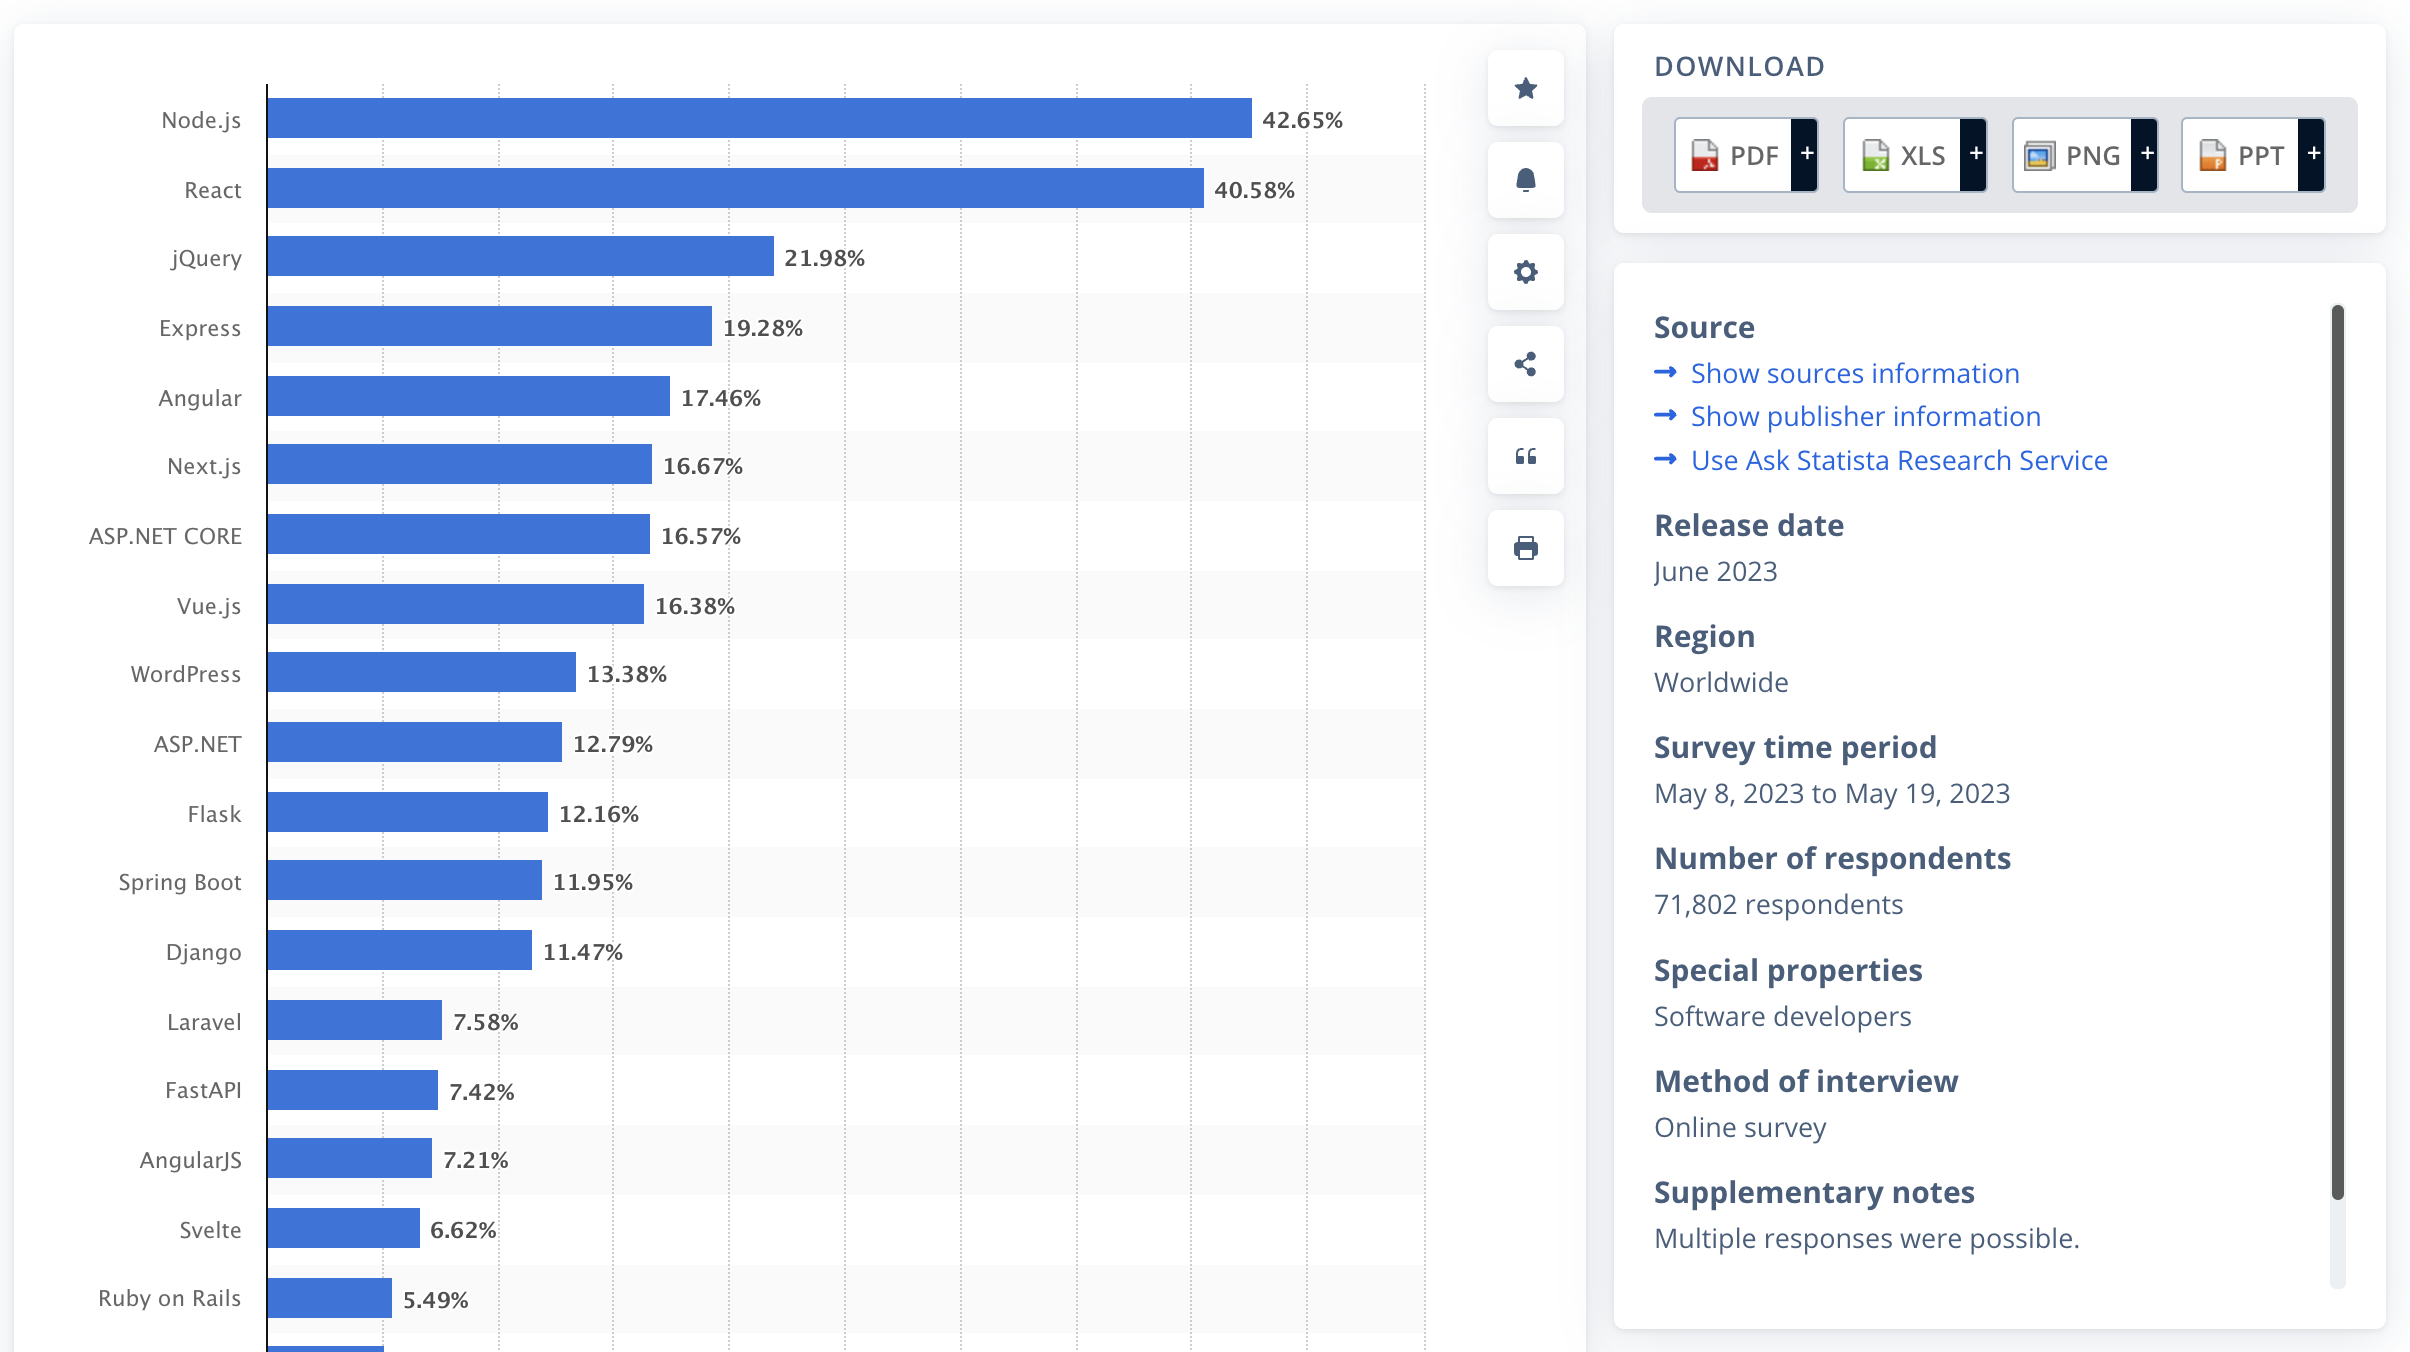
\includegraphics[width=0.8\textwidth]{aulas/aula1-statistica.png}
    \caption{Frameworks mais usados}
  \end{figure}
\end{frame}
\begin{frame}[fragile]
  \frametitle{Aprofundamento e Recursos Complementares}
  \textbf{Superando o Desafio do Tempo Limitado}
  \begin{itemize}
    \item \textit{68 horas de aula} são um ponto de partida. Para aprofundar, utilizaremos tutoriais e vídeos selecionados, permitindo que os alunos explorem os tópicos de interesse mais a fundo.
    \item \textit{Temas de Aprofundamento:} Incluem uso avançado de Git, integração de bibliotecas de terceiros, técnicas de deploy e hospedagem, além de práticas recomendadas para desenvolvimento com frameworks modernos.
    \item \textit{Preparação para o Mercado:} A combinação de React.js e Node.js é altamente valorizada na indústria, preparando os alunos para oportunidades em desenvolvimento frontend e full-stack.
  \end{itemize}
\end{frame}


\begin{frame}[fragile]
  \frametitle{Semana 1: Introdução à Web, Arquitetura Cliente-Servidor e Ferramentas de Versionamento}
  \textbf{Tópicos:}
  \begin{itemize}
    \item História da Web, conceitos de Internet e Web, arquitetura cliente-servidor.
    \item Introdução ao Git e GitHub.
  \end{itemize}
  \textbf{Estudo Complementar:}
  \begin{itemize}
    \item Configuração de um ambiente de desenvolvimento, instalação do Git, criação de um repositório no GitHub.
  \end{itemize}
\end{frame}

\begin{frame}[fragile]
  \frametitle{Semana 2: Revisão dos Protocolos Web}
  \textbf{Tópicos:}
  \begin{itemize}
    \item HTTP, HTTPS, WebSockets.
  \end{itemize}
  \textbf{Estudo Complementar:}
  \begin{itemize}
    \item Exploração de requisições HTTP utilizando Postman ou ferramentas similares.
  \end{itemize}
\end{frame}

\begin{frame}[fragile]
  \frametitle{Semana 3: Linguagens de Marcação e Introdução ao HTML5}
  \textbf{Tópicos:}
  \begin{itemize}
    \item Estrutura básica do HTML, formulários, links, e multimídia.
  \end{itemize}
  \textbf{Estudo Complementar:}
  \begin{itemize}
    \item Criação de uma página simples utilizando HTML5.
  \end{itemize}
\end{frame}

\begin{frame}[fragile]
  \frametitle{Semana 4: CSS e Estilização}
  \textbf{Tópicos:}
  \begin{itemize}
    \item Seletores, propriedades, box model, flexbox.
  \end{itemize}
  \textbf{Estudo Complementar:}
  \begin{itemize}
    \item Prática de estilização de uma página HTML com CSS puro.
  \end{itemize}
\end{frame}

\begin{frame}[fragile]
  \frametitle{Semana 5: JavaScript e TypeScript Básicos}
  \textbf{Tópicos:}
  \begin{itemize}
    \item Sintaxe básica, tipos, estruturas de controle, funções.
  \end{itemize}
  \textbf{Estudo Complementar:}
  \begin{itemize}
    \item Conversão de um script simples de JavaScript para TypeScript.
  \end{itemize}
\end{frame}

\begin{frame}[fragile]
  \frametitle{Semana 6: Primeira Avaliação Teórica e Introdução ao React.js}
  \textbf{Tópicos:}
  \begin{itemize}
    \item Criação de componentes simples com React.js e TypeScript.
  \end{itemize}
\end{frame}

\begin{frame}[fragile]
  \frametitle{Semana 7: React.js e Componentes}
  \textbf{Tópicos:}
  \begin{itemize}
    \item JSX, props, state, ciclo de vida dos componentes.
  \end{itemize}
  \textbf{Estudo Complementar:}
  \begin{itemize}
    \item Construção de componentes reutilizáveis com React.
  \end{itemize}
\end{frame}

\begin{frame}[fragile]
  \frametitle{Semana 8: Modularização e Reutilização de Componentes}
  \textbf{Tópicos:}
  \begin{itemize}
    \item Importação, exportação de componentes, composição vs herança.
  \end{itemize}
  \textbf{Estudo Complementar:}
  \begin{itemize}
    \item Estudo de caso de modularização em um projeto React.
  \end{itemize}
\end{frame}

\begin{frame}[fragile]
  \frametitle{Semana 9: Estilização Avançada e Design Responsivo}
  \textbf{Tópicos:}
  \begin{itemize}
    \item CSS in JS, bibliotecas como Styled-components, media queries.
  \end{itemize}
  \textbf{Estudo Complementar:}
  \begin{itemize}
    \item Aplicação de Styled-components em componentes React.
  \end{itemize}
\end{frame}

\begin{frame}[fragile]
  \frametitle{Semana 10: Usabilidade e Acessibilidade}
  \textbf{Tópicos:}
  \begin{itemize}
    \item Melhores práticas, ferramentas de teste de acessibilidade.
  \end{itemize}
  \textbf{Estudo Complementar:}
  \begin{itemize}
    \item Análise de acessibilidade em um site com ferramentas online.
  \end{itemize}
\end{frame}

\begin{frame}[fragile]
  \frametitle{Semana 11: Padrões para Interoperabilidade de Dados}
  \textbf{Tópicos:}
  \begin{itemize}
    \item JSON, XML, APIs RESTful.
  \end{itemize}
  \textbf{Estudo Complementar:}
  \begin{itemize}
    \item Prática de consumo de APIs RESTful com React e TypeScript.
  \end{itemize}
\end{frame}

% Continue com este padrão para as semanas restantes...

\begin{frame}[fragile]
  \frametitle{Semana 12-13: Projeto Prático em React.js e TypeScript}
  \textbf{Tópicos:}
  \begin{itemize}
    \item Aplicação dos conhecimentos adquiridos em um projeto prático, integração com API REST.
  \end{itemize}
  \textbf{Estudo Complementar:}
  \begin{itemize}
    \item Documentação de APIs REST utilizadas no projeto.
  \end{itemize}
\end{frame}

\begin{frame}[fragile]
  \frametitle{Semana 14: Apresentação dos Projetos}
  \textbf{Atividade:}
  \begin{itemize}
    \item Apresentação e avaliação dos projetos desenvolvidos pelos alunos.
  \end{itemize}
\end{frame}

\begin{frame}[fragile]
  \frametitle{Semana 15: Segunda Avaliação Teórica e Introdução a Arquitetura de Software}
  \textbf{Tópicos da Aula:}
  \begin{itemize}
    \item Estilos arquiteturais mais usados na Web.
  \end{itemize}
\end{frame}

\begin{frame}[fragile]
  \frametitle{Semana 16: Arquitetura de Software e Estilos Arquiteturais}
  \textbf{Tópicos:}
  \begin{itemize}
    \item MVC, SPA, MPA, vantagens e desvantagens.
  \end{itemize}
  \textbf{Estudo Complementar:}
  \begin{itemize}
    \item Análise de um projeto React sob o ponto de vista arquitetural.
  \end{itemize}
\end{frame}

\begin{frame}[fragile]
  \frametitle{Semana 17: Avaliação Prática}
  \textbf{Atividade:}
  \begin{itemize}
    \item Avaliação prática em laboratório, aplicando conhecimentos adquiridos ao longo do curso.
  \end{itemize}
\end{frame}

\begin{frame}[fragile]
  \frametitle{Semana 18: Prova Optativa}
  \textbf{Atividade:}
  \begin{itemize}
    \item Oferecida para alunos que necessitam melhorar suas notas.
  \end{itemize}
\end{frame}


\begin{frame}[fragile]
  \frametitle{Metodologia de Ensino}
  \begin{itemize}
    \item Aulas teóricas interativas com exposições dialogadas, utilizando projetor e quadro para promover o envolvimento dos alunos.
    \item Práticas de laboratório com exercícios dirigidos e projetos de desenvolvimento web, proporcionando experiência prática com supervisão.
    \item Estudos de caso para análise e discussão em sala, aplicando conceitos a situações reais de desenvolvimento web.
    \item Avaliação contínua através de feedback instantâneo, quizzes, e pequenos testes para monitorar o progresso e entender necessidades de reforço.
  \end{itemize}
\end{frame}
\begin{frame}[fragile]
  \frametitle{Tarefa de Casa: Configuração do Ambiente de Desenvolvimento}
  \textbf{Preparação Inicial para o Desenvolvimento Web Moderno}
  \begin{itemize}
    \item \textbf{Escolha do Sistema Operacional:}
    \begin{itemize}
      \item Opte por \textit{Ubuntu Linux} como seu sistema operacional para desenvolvimento. A configuração do Node.js pode ser mais desafiadora no Windows devido a peculiaridades de sistema.
    \end{itemize}
    
    \item \textbf{Instalação do Node.js:}
    \begin{itemize}
      \item Instale o Node.js para executar e desenvolver aplicações JavaScript do lado do servidor. Siga as instruções oficiais em: \url{https://nodejs.org/en/download/package-manager/}
    \end{itemize}
    
    \item \textbf{Instalação do Visual Studio Code (VSCode):}
    \begin{itemize}
      \item Instale o VSCode, um editor de código fonte leve e poderoso, suportando desenvolvimento Node.js, JavaScript e TypeScript. Disponível em: \url{https://code.visualstudio.com/}
    \end{itemize}
    
    \item \textbf{Criação de Conta no GitHub:}
    \begin{itemize}
      \item Para quem ainda não tem, crie sua conta no GitHub, essencial para controle de versão e colaboração em projetos de software. Visite: \url{https://github.com/}
    \end{itemize}
  \end{itemize}
\end{frame}
